\section{Propagation of Means and Covariances}
In practice we are often more interested in linear functions of the random variables than
the random variables themselves. The most often encountered examples are covered by the linear transformation
\begin{equation*}
Y=BX+K,
\end{equation*}
where B is a known m by n matrix and k (also known) is m by 1. The linearity of the
expectation operator E yields
\begin{equation}
E\{Y\}=E\{BX+K\}=B\,E\{X\}+k.
\end{equation}
Then the covariance for Y comes from the covariance for X. This formula is highly important, and we will use it often !

Law of Covariance Propagation If Y = BX + k  and k is known then
\begin{equation}
\Sigma_Y=B\Sigma_XB^T.
\end{equation}
The proof is direct. The shift by k cancels itself in $Y-E\{Y\}$, and the matrix B comes
outside by linearity:
\begin{equation*}
\begin{split}
\Sigma_Y&=E\{(Y-E\{Y\})(Y-E\{Y\})^T\}\\
&=E\{(BX+k-BE\{X\}-k)(BX+k-BE\{X\}-k)^T\}\\
&=E\{(BX-BE\{X\})(BX-BE\{X\})^T\}\\
&=BEE\{(X-E\{X\})(X-E\{X\})^T\}B^T=B\Sigma_XB^T.\\
\end{split}
\end{equation*} 
In geodesy, $\Sigma_Y=B\Sigma_XB^T$ the law appears in many applications. Sometimes B gives
a change of coordinates (in this case B is square). For least squares, X contains the n
observations and Y contains the m fitted parameters (in this case B is rectangular, with
m $>$n). We will frequently quote this law of covariance propagation.

In the special case that all $X_i$; are independent, $\Sigma_X$ is diagonal. Furthermore, if B is 1 by n and hence $Y=b_1X_1+\cdots+b_nX_n$, one obtains the law of error propagation: 
\begin{equation}
\sigma^2_Y=b^2_1\sigma^2_1+\cdots+b^2_n\sigma^2_n.
\end{equation}
This gives the variance $\sigma^2_Y$ for a combination of n independent measurements.

If the vector k is also subject to error, independently of X and with mean zero, its
covariance matrix $\Sigma_k$ would be included in the covariance of Y = BX + k:
\begin{equation*}
\Sigma_Y=B\Sigma_XB^T+\Sigma_k.
\end{equation*}
This law is at the heart of the Kalman filter.

Now come examples from positioning.

Example 4.10\; In leveling it is common practice to attribute the variance $\sigma^2_0$ to a leveling observation of length l. According to equation (4.72), in leveling lines of lengths 2l, . . . , nl we have variances $2\sigma^2_0,...,n\sigma^2_0$. Consequently the weights are 1/2,...,1/n. For a leveling line observed under these conditions the weight is reciprocal to the distance.

\begin{figure}[h]
	\centering
	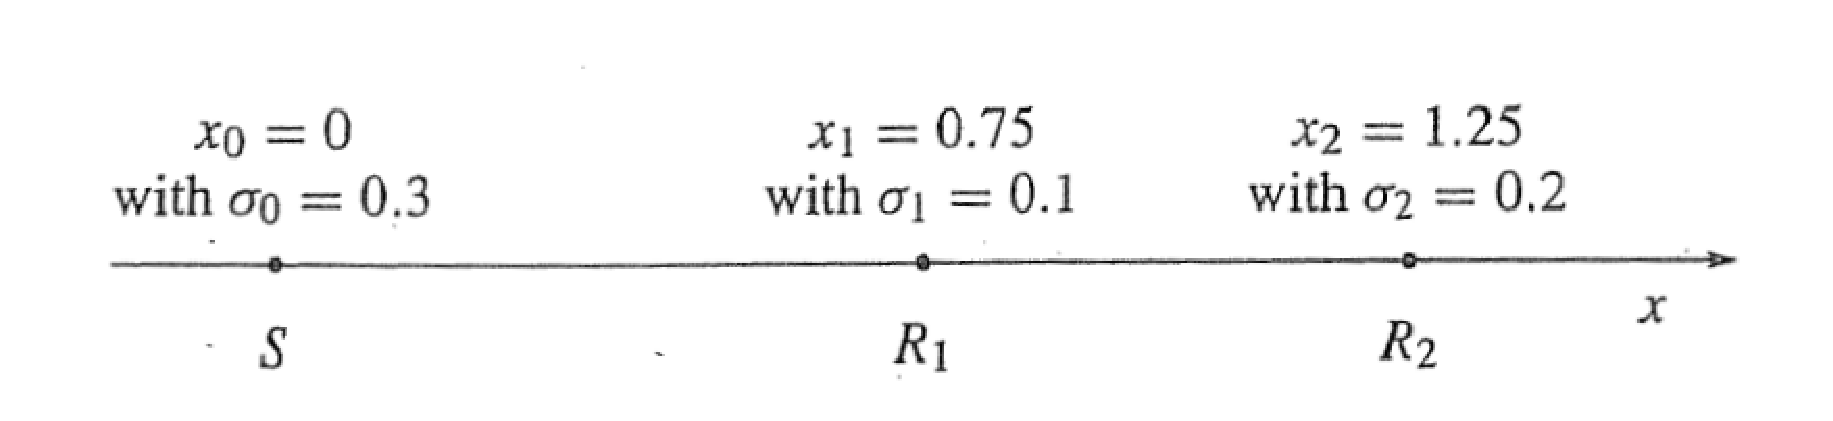
\includegraphics[width=0.7\linewidth]{TeX_files/Part02/chapter04/image/4-8}
	\caption{Figure 4.8\; Pseudoranges from the satellite S to the receivers $R_1$ and $R_2$}
	\label{fig:4-8}
\end{figure}
Example 4.11\; We have two independent random variables x and y with zero mean and variance 1. For fixed c the linear expression z = ax + by + c has a normal distribution with mean c and variance $a^2+b^2:\Sigma_z=[a\;b]\begin{bmatrix}1 & 0\\0 & 1\end{bmatrix}
\begin{bmatrix} a\\b \end{bmatrix}=a^2+b^2$.
Example 4.12\; A basic example to surveying is the coordinate transformation from polar
to Cartesian coordinates:
\begin{equation*}
x=rcos\theta \quad and \quad y=rsin\theta
\end{equation*}
From given values of $(r,\theta)$ the coordinates (x,y) are found immediately. For given variances $(\sigma_r,\sigma_\theta)$, the propagation law yields $\sigma_x$ and $\sigma_y$ by linearization. The matrix B becomes tht Jacobian matrix J containing the partial derivatives:
\begin{equation*}
J=
\begin{bmatrix}
\partial x/\partial r & \partial x/\partial \theta\\
\partial y/\partial r & \partial y/\partial \theta
\end{bmatrix}
=
\begin{bmatrix}
cos\theta &-rsin\theta \\
sin\theta &rcos\theta.
\end{bmatrix}
\end{equation*}
The law of propagation of variances yields the covariance matrix $\Sigma_x$ for x = (x,y):
\begin{equation*}
\Sigma_x=J
\begin{bmatrix}
\sigma^2_r & 0 \\
0 &\sigma^2_\theta
\end{bmatrix}
J^T=
\begin{bmatrix}
\sigma^2_rcos^2\theta+r^2\sigma^2_\theta sin^2\theta & (\sigma^2_r-r^2\sigma^2_\theta)sin\theta cos\theta\\
(\sigma^2_r-r^2\sigma^2_\theta)sin\theta cos\theta &
\sigma^2_rsin^2\theta+r^2\sigma^2_\theta cos^2\theta 
\end{bmatrix}
\end{equation*}
Insertion of the actual values yields the covariance matrix $\Sigma_x$. The x and y coordinates are uncorrelated when $\theta=0$ or $\theta=\pi/4$. Then we have a polar point determination in the direction of one of the coordinate axes. Also $\sigma_{xy}=0$ when the special condition $\sigma^2_r=r^2\sigma^2_\theta$ prevails. Then the standard deviation $\sigma_r$ of the distance measurement equals the perpendicular error $r\sigma_\theta$. This leads to circular confidence ellipses.

Example 4.13\; Single differences of pseudoranges One of the best illustrations of the
covariance propagation law is the process of taking differences. The difference of two
receiver positions is the baseline vector between them. So we are solving for this difference $(x_2-x_1)$ rather than the individual coordinates $x_1$ and $x_2$. Of course the difference operator is linear, given by a simple 1 by 2 matrix [-1 1]. The hope is that the difference is more stable than the separate positions. The covariance matrix should be smaller.

This example is in one dimension. The satellite and the two receivers in Figure 4.8
are exactly on a line, which never happens in practice. A later example (Section 10.3) will
have two satellites and two receivers and work with double differences.

Physically, taking the difference cancels the sources of error that are common to
both receivers (the satellite clock error and almost all of the ionospheric delay). This is
the basis for Differential GPS. There are many applications of DGPS, coming in Part III
of this book. If one of the receiver positions is well established (the home base), then an accurate baseline gives an accurate position for the second receiver (the rover). Differential GPS allows us to undo the dithering of the satellite clock. Our goal here is to see how the difference (the baseline) can be more accurate than either endpoint—and to calculate its covariance by the propagation law.

\begin{figure}[h]
	\centering
	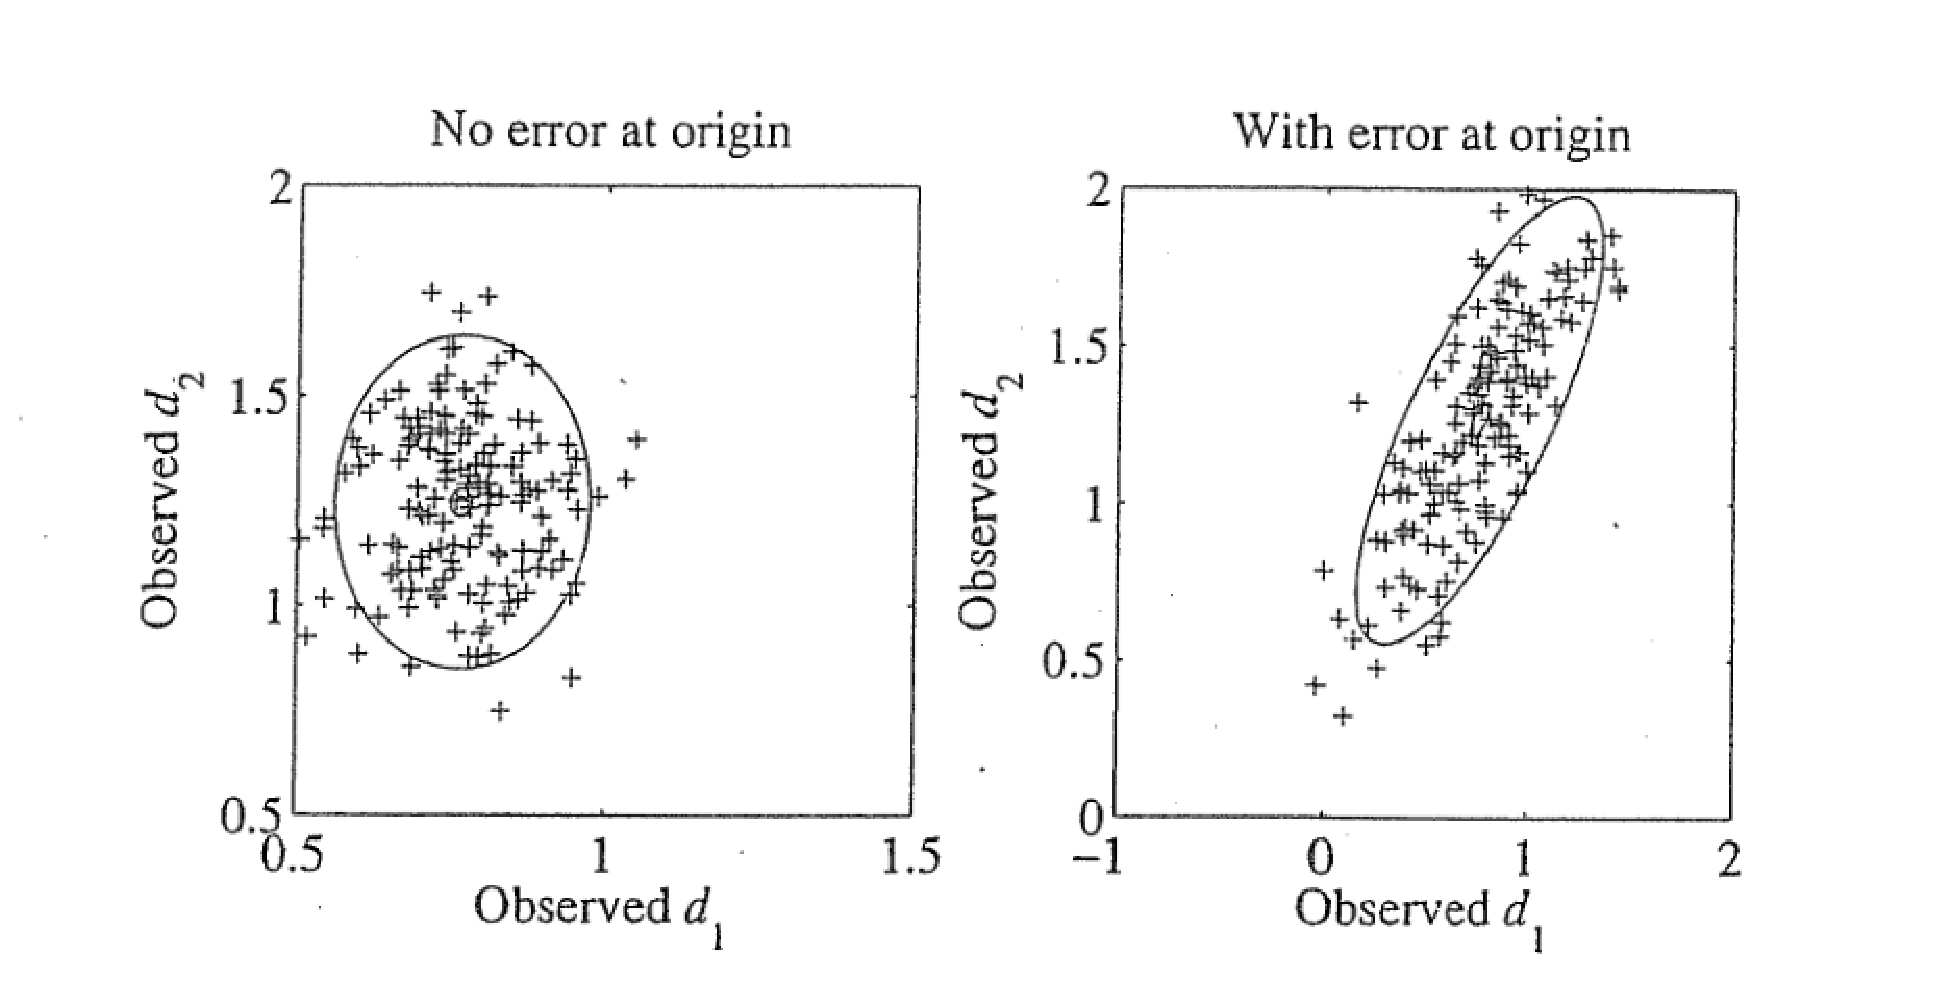
\includegraphics[width=0.7\linewidth]{TeX_files/Part02/chapter04/image/4-9}
	\caption{Figure 4.9 The one-dimensional normal distribution and the $2\sigma$-curve of confidence}
	\label{fig:4-9}
\end{figure}

We can use the MATLAB command randn (1,100) to produce 100 explicit sample points $(d_1,d_2)$. Then the covariance matrices can be illustrated by Figure 4.9, and by the
very simple M-file oned. We owe the example and also its M-file to Mike Bevis. First
come the formulas.

The positions of the satellite and the receivers are $x_0=0,x_1=0.75,x_2=1.25$.
Those positions are subject to independent random errors, normally distributed with mean
zero and standard deviations $\sigma_0=0.3,\sigma_1=0.1,\sigma_2=0.2$. We chose ao largest to make the figures clear. The measurement of $x_1$ (its pseudorange) has errors from the satellite and that first receiver. A vector of n samples is defined as 
\begin{equation*}
\rho_1=0.75\ast ones(1,n)+\sigma_1\ast randn(1,n)-\sigma_0\ast randn(1,n).
\end{equation*}
A similar command gives n samples of the pseudorange $\rho_2$. But since randn produces
new numbers every time, we must define $del = \sigma_0\ast randn(1,n)$ and subtract that same satellite error from both $\rho_1$ and $\rho_2$. This is the whole point (!), that the difference eliminates the satellite error. The M-file achieves this by $\sigma_0=0$, or we can work directly with $\rho_2-\rho_1$.

Now come the covariance matrices. We use the important fact that the mean(the
average) of n samples has variance (and covariance) reduced by 1/n. Thus from the data
we compute the scalars
\begin{equation*}
m_1=mean(\rho_1) \quad and \quad m_2=mean(\rho_2)\\
\end{equation*}
\begin{equation*}
V=cov(\rho_1,\rho_2)  \quad and \quad V_m=V/n=covariance\, of\, the\, sample\, mean. 
\end{equation*}
The first plot in Figure 4.9 shows the n sample values of $(\rho_1,\rho_2)$, centered about the mean $(m_1, m_2)$. The small inner ellipse is controlled by Vm and the outer ellipse by $V_m$. On average 86\% of the sample points should lie in that outer ellipse with nsigma set to 2.

The key point is that $\rho_1$ is correlated with $\rho_2$. Therefore the ellipses are tilted. The same satellite error enters both $\rho_1$ and $\rho_2$, with the same sign. The correlation is positive. The errors are large because of $\sigma_0=0.3$. The theoretical covariance matrix $\Sigma$ and the sample covariance matrix V are
\begin{equation*}
\Sigma=
\begin{bmatrix}
\sigma^2_1 & \sigma_{12}\\
\sigma_{12} & \sigma^2_2
\end{bmatrix}
\quad and \quad
V_{ij}=(\rho_i-m_i)^T(\rho_i-m_j).
\end{equation*} 
Now take differences $d=\rho_2-\rho_1$. The linear transformation is T=[-1 1]. The
propagation law $T\Sigma T^T$ says that the covariance (or just variance) of the scalar d should be
\begin{equation*}
covariance=\Sigma_d=[-1\; +1]\Sigma
\begin{bmatrix} -1\\+1 \end{bmatrix}
=\sigma^2_1-2\sigma_{12}+\sigma^2_2.
\end{equation*}
Notice how the effect of $\sigma_0=0.3$ has disappeared from $\Sigma_d$. For the sample value $V_d$ of the covariance of d we compute around the sample mean $m_d$:
\begin{equation*}
m_d=mean(d) \quad and \quad
V_d=cov(d)=\sum^n_1(d(i)-m_d)^2.
\end{equation*} 
The MATLAB output compares the predicted $\Sigma_d$ with the actual $V_d$.

One more plot is of great interest. It shows the measured distances $d_1$ and $d_2$ to the
receivers, without the satellite error that they share:
\begin{equation*}
d_1=0.75\ast ones(1,n)+\sigma_1\ast randn(1,n)
\end{equation*}
\begin{equation*}
d_2=1.25\ast ones(1,n)+\sigma_2\ast randn(1,n).
\end{equation*}
Figure 4.9\; (right) shows the n points $(d_1,d_2)$, with the sample mean $m_{d_1,d_2}$ and the sample covariance $V_{d_1,d_2}$. The error ellipse is now aligned with the axes: no correlation now.
Taking differences has decorrelated the errors in $d_1$ from the errors in $d_2$. The theoretical
covariance matrix for $(d_1,d_2)$ is diagonal:
\begin{equation*}
\begin{bmatrix}
\sigma^2_1 & 0 \\
0  & \sigma^2_2
\end{bmatrix}.
\end{equation*}
This example verifies experimentally the propagation law. We used that law for $\Sigma_d=T\Sigma T^T$. The samples of $d_2-d_1$ give the experimental value of this covariance . The probability is very high that it is close to $\Sigma_d$.

As a final curiosity, consider two satellites and receivers all on the x axis. For satellites 1 and 2 we can use single differences $d^1$ and $d^2$ as above. But the double difference
$d^1-d^2$ from all four measurements is automatically zero. The measurements $\rho^2_1$ and $\rho^2_2$ to the second satellite both include the distance s between satellites, and everything cancels in the double difference:
\begin{equation*}
\begin{split}
d^1-d^2&=(\rho^1_1-\rho^1_2)-(\rho^2_1-\rho^2_2)\\
&=(\rho^1_1-\rho^1_2)-(\rho^1_1+s-\rho^1_2-s)=0.
\end{split}
\end{equation*}
In two or three dimensions this will not occur! Length is nonlinear; we have differences of
square roots. Satellites and receivers are not collinear. Double differencing is the fundamental tool in Chapter 10 on processing of GPS data.

Example 4.14\; Variance of local east-north-up coordinates from GPS The relationship
between increments of geocentric coordinates (x,y,z) and of the local east-north-up coordinates
(e,n,u) is determined by the latitude and longitude in the Jacobian F:
\begin{equation}
\begin{bmatrix}
e\\ n\\ u
\end{bmatrix}
=
\begin{bmatrix}
-sin\lambda & cos\lambda & 0\\
-sin\varphi cos\lambda & -sin\varphi sin\lambda & cos\varphi \\
cos\varphi cos\lambda & cos\varphi sin\lambda & sin\varphi
\end{bmatrix}
\begin{bmatrix}
x\\y\\z
\end{bmatrix}
=F
\begin{bmatrix}
x\\y\\z
\end{bmatrix}.
\end{equation} 
We want to compute the covariance matrix for e,n,u. It is based on a given covariance
matrix $\Sigma_{xyz}$ for the geocentric coordinate increments in x,y,z. The law of propagation of
covariances (4.71) gives
\begin{equation}
\Sigma_{enu}=F\Sigma_{xyz}F^T.
\end{equation}
A covariance matrix from practice, with units of $mm^2$, is
\begin{equation*}
\Sigma_{xyz}=
\begin{bmatrix}
25 & -7.970 &18.220\\
-7.970 & 4 & -6.360\\
18.220 & -6.360 &16
\end{bmatrix}.
\end{equation*}
The position is $\varphi=55^。54'$, $\lambda=12^。29$, so the coordinate change matrix is
\begin{equation*}
F=
\begin{bmatrix}
-0.216 & 0.976 &0\\
-0.808 & -0.179 & 0.561\\
0.547 &0.121&0.824
\end{bmatrix}.
\end{equation*}
Hence the covariance matrix for the coordinate increments (e,n,u) becomes
\begin{equation*}
\Sigma_{enu}=
\begin{bmatrix}
8.34 & 3.96 &-14.90\\
3.96 & 3.95 &-8.24\\
-14.90 &-8.24 &32.52
\end{bmatrix}.
\end{equation*}
The standard deviations are $\sigma_e=2.9mm$, $\sigma_n=2.0mm$ and $\sigma_u=5.7mm$. These numbers
are in good agreement with experience. The vertical deviation $\sigma_u=\sigma_{up}$ is about twice as large as the in-plane deviations. 
